O campus do Gama da Universidade de Brasília, construído entre os anos de 2009 a 2011, localizado na Área Especial de Indústria Projeção A, UnB - Setor Leste Gama, Brasília-DF, possui área total de 335074 $m^2$, com área construída de 16009 $m^2$, sendo projetada para abrigar no total, cinco cursos de engenharia, sendo eles de Aeroespacial, Automotiva, Eletrônica, Energia e Software.

\begin{figure}[H]
  \centering
  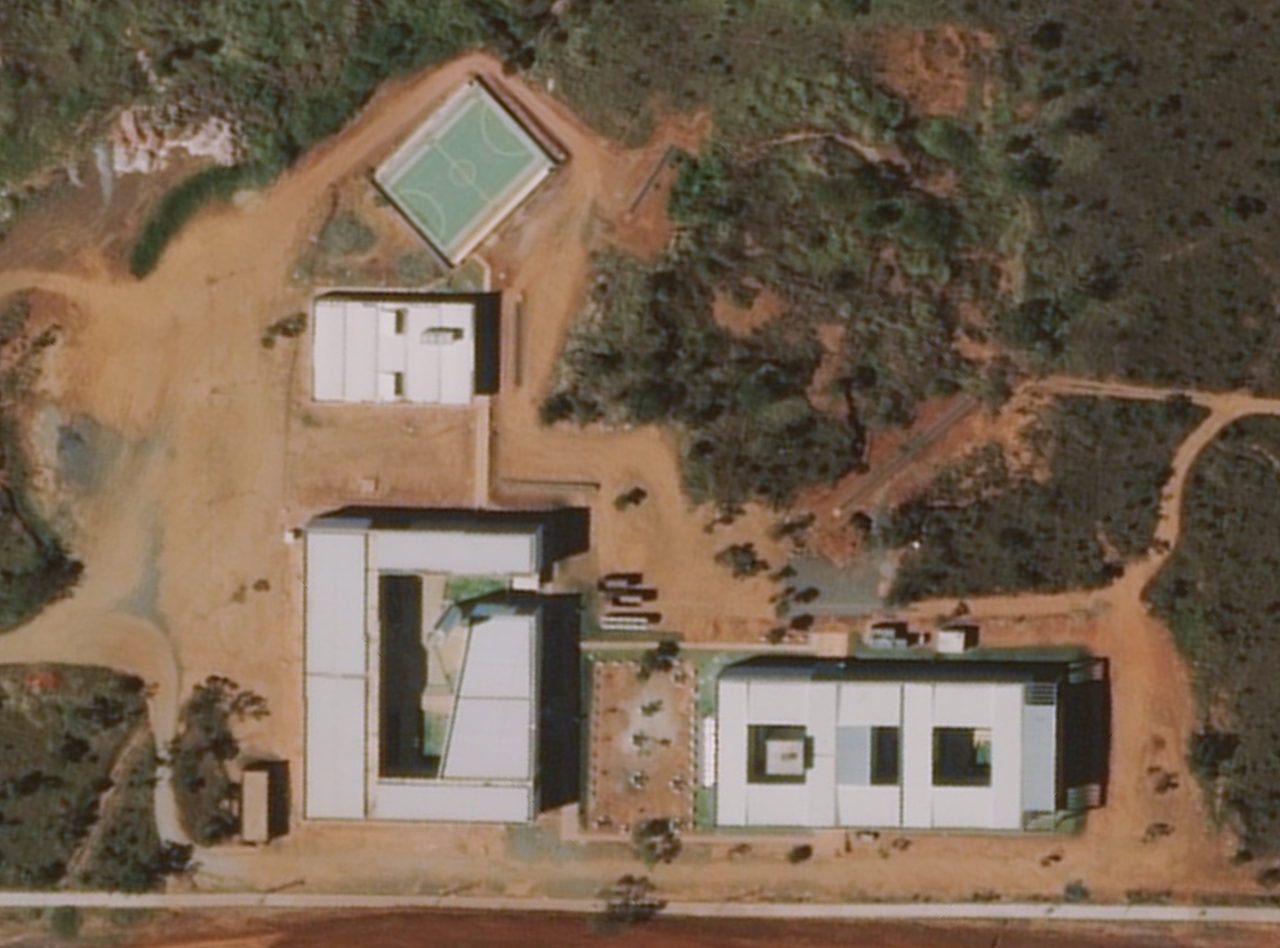
\includegraphics[width=0.87\textwidth]{figuras/fga1}
  \caption{Vista aérea do campus UnB Gama. Em destaque os prédios já construídos.}
  \label{img:fga1}
\end{figure}

Em 2013, segundo informações do DaEng, sete meses após o início da gestão do Diretório Acadêmico do Gama , iniciaram-se medidas para a implementação do cercamento do campus. Contudo, mediante a falta de documentos legais, como licenciamento ambiental e demarcação de terras, o processo de licitação teve de ser adiado e, somente em meados do ano de 2015 as obras foram iniciadas.
Diante disso, durante os anos de 2012 até os dias atuais, muitos alunos, professores e comunidade em geral que frequentam a Faculdade do Gama vêm enfrentando uma rotina de roubos a carros na área do estacionamento do campus, cujo principal fator seria a da falta de um cercamento, com guaritas, que possibilitassem o controle de pessoas que acessam o local.
Como maneira de obter alguns dados referentes à mobilidade de alunos, professores e comunidade até o campus, o Grupo 1 da disciplina Projeto Integrador 1 decidiu aplicar uma pesquisa sobre o meio de transporte utilizado para descolamento residência-campus,   quantas vezes o veículo foi roubado, se o indivíduo prestou alguma queixa formal (boletim de ocorrência) e o(s) ano(s) do ocorrido, caso este utilize automóvel para locomoção. A pesquisa foi elaborada no aplicativo \textit{Google Drive- Formulários} e publicada no período do dia 02 de agosto de 2015 ao dia 29 de agosto do mesmo ano no grupo destinado aos alunos e professores da UnB-Gama na rede social \textit{Facebook}. Durante este período, em parte, 93 pessoas responderam às seis questões propostas no questionário, resultando nos dados apresentados nos gráficos a seguir.

\begin{figure}[H]
  \centering
  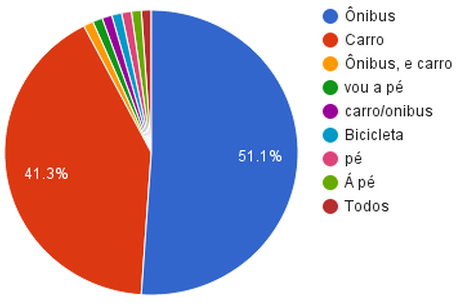
\includegraphics[width=0.75\textwidth]{figuras/pesquisa}
  \caption{Pesquisa de mobilidade dos alunos da FGA. Fonte: Google Drive-Formulários, 2015.}
  \label{img:pesquisa}
\end{figure}
 
O [Grafico \ref{img:pesquisa}] apresenta a distribuição, no espaço amostral, dos meios  de transporte utilizados. Mais da metade dos alunos utilizam apenas ônibus para locomoção, 51,1\%, tendo 41,3\% utilizando apenas o carro como meio de transporte, sendo os 7,6\% restantes divididos entre locomoção a pé, bicicleta, ônibus e carro.Apresenta-se, então, uma significativa frota de carros diária no campus, demandando maiores investimentos para segurança destes bens. 
